% Hashgrid bilinear-lookup + feature vector with curving arrows.
% Two cells (blue coarse / green fine), each with its bilinear sample,
% then curving arrows out to a narrow vertical feature column made of
% 8 stacked squares: 2 blue, 2 green, 2 yellow, 2 red (top -> bottom).
\documentclass[tikz,border=4pt]{standalone}
\usepackage{tikz}
\usepackage{amsmath}
\usepackage{amssymb}
\usepackage{xcolor}
\usetikzlibrary{positioning, calc, arrows.meta}

\begin{document}
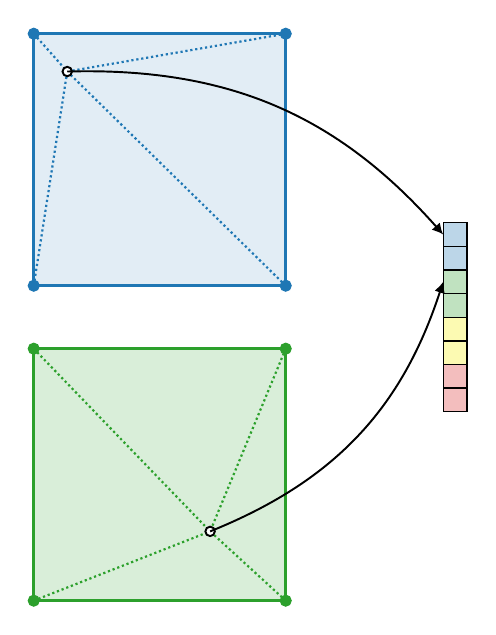
\begin{tikzpicture}[
  font=\sffamily\footnotesize,
  >={Latex[length=4pt,width=4pt]},
]
\definecolor{cgridA}{HTML}{1F77B4}   % blue base  (cell border / corners)
\definecolor{cgridB}{HTML}{2CA02C}   % green base (cell border / corners)
\definecolor{cLemon}{HTML}{F4ED00}   % lemon yellow base (for swatch 34)
\definecolor{cRedB} {HTML}{D62728}   % red base (for swatch 19)
% Feature swatches (palette indices):
%   4  = Blue  !30!white
%   9  = Green !30!white
%   34 = Lemon !30!white
%   19 = Red   !30!white

\pgfmathsetmacro{\sz}{3.2}

% =====================================================================
% Blue (coarse) cell — TOP
% =====================================================================
\begin{scope}[shift={(0,4.0)}]
  \fill[cgridA, opacity=0.13] (0,0) rectangle (\sz,\sz);
  \draw[cgridA, line width=1.1pt] (0,0) rectangle (\sz,\sz);
  \pgfmathsetmacro{\sx}{0.133*\sz}
  \pgfmathsetmacro{\sy}{0.850*\sz}
  \coordinate (sB) at (\sx,\sy);
  \draw[cgridA, densely dotted, line width=0.8pt] (0,0)    -- (sB);
  \draw[cgridA, densely dotted, line width=0.8pt] (\sz,0)  -- (sB);
  \draw[cgridA, densely dotted, line width=0.8pt] (0,\sz)  -- (sB);
  \draw[cgridA, densely dotted, line width=0.8pt] (\sz,\sz)-- (sB);
  \foreach \p in {(0,0),(\sz,0),(0,\sz),(\sz,\sz)} {
    \filldraw[cgridA] \p circle (0.07);
  }
  \draw[black, line width=0.7pt, fill=white] (sB) circle (0.06);
\end{scope}

% =====================================================================
% Green (fine) cell — BOTTOM
% =====================================================================
\begin{scope}[shift={(0,0)}]
  \fill[cgridB, opacity=0.18] (0,0) rectangle (\sz,\sz);
  \draw[cgridB, line width=1.1pt] (0,0) rectangle (\sz,\sz);
  \pgfmathsetmacro{\sx}{0.700*\sz}
  \pgfmathsetmacro{\sy}{0.275*\sz}
  \coordinate (sG) at (\sx,\sy);
  \draw[cgridB, densely dotted, line width=0.8pt] (0,0)    -- (sG);
  \draw[cgridB, densely dotted, line width=0.8pt] (\sz,0)  -- (sG);
  \draw[cgridB, densely dotted, line width=0.8pt] (0,\sz)  -- (sG);
  \draw[cgridB, densely dotted, line width=0.8pt] (\sz,\sz)-- (sG);
  \foreach \p in {(0,0),(\sz,0),(0,\sz),(\sz,\sz)} {
    \filldraw[cgridB] \p circle (0.07);
  }
  \draw[black, line width=0.7pt, fill=white] (sG) circle (0.06);
\end{scope}

% =====================================================================
% Feature column — 8 stacked squares, centered vertically between cells.
%   - The cells span y ∈ [0, 7.2] (each is 3.2 tall, gap = 0.8).
%   - Vertical midpoint: y = 3.6.
%   - Square side = 0.30 cm  (~2× corner-marker diameter of 0.14 cm).
%   - Total stack height = 8 × 0.30 = 2.4 cm  → from y=2.4 to y=4.8.
%   - Column x: 5.20 to 5.50.
% =====================================================================
\pgfmathsetmacro{\fw}{0.30}                         % cell side
\pgfmathsetmacro{\fxL}{5.20}                        % left x of column
\pgfmathsetmacro{\fxR}{\fxL + \fw}
\pgfmathsetmacro{\fyTop}{4.80}                      % top y of column
\pgfmathsetmacro{\fyBot}{\fyTop - 8*\fw}            % bottom y of column
\pgfmathsetmacro{\fxc}{0.5*(\fxL+\fxR)}             % column center x

% Top -> bottom: 2 Blue (swatch 4), 2 Green (9), 2 Lemon (34), 2 Red (19).
\foreach \i/\col in {0/cgridA, 1/cgridA,
                      2/cgridB, 3/cgridB,
                      4/cLemon, 5/cLemon,
                      6/cRedB,  7/cRedB}{
  \pgfmathsetmacro{\fyHi}{\fyTop - \i*\fw}
  \pgfmathsetmacro{\fyLo}{\fyHi - \fw}
  \fill[\col!30!white] (\fxL,\fyLo) rectangle (\fxR,\fyHi);
  \draw[black, line width=0.5pt] (\fxL,\fyLo) rectangle (\fxR,\fyHi);
}

% Targets for incoming arrows = left-mid of TOP-MOST blue and FIRST green squares.
\pgfmathsetmacro{\tBlueY}{\fyTop - 0.5*\fw}             % center of top blue cell
\pgfmathsetmacro{\tGreenY}{\fyTop - 2.5*\fw}            % center of first green cell
\coordinate (tBlue)  at (\fxL,\tBlueY);
\coordinate (tGreen) at (\fxL,\tGreenY);

% =====================================================================
% Curving arrows from the two sample points to the feature targets.
% =====================================================================
% Single-sided C-curves (blue arches up, green arches down).
\draw[->, black, line width=0.7pt]
  (sB) to[bend left=25, looseness=1.0]  (tBlue);
\draw[->, black, line width=0.7pt]
  (sG) to[bend right=25, looseness=1.0] (tGreen);

\end{tikzpicture}
\end{document}
